\documentclass[c,unicode,russian]{beamer}
\usepackage{hyperref}
\usepackage{alltt}
\usepackage{verbatim}
\usepackage{fancyvrb}

\usepackage{fontspec}
\setsansfont{Ubuntu}
\setmonofont{Ubuntu Mono}
\usepackage{polyglossia}
\setdefaultlanguage{russian}

\useinnertheme{metropolis}
\useoutertheme{metropolis}
\usecolortheme{metropolis}

\usepackage{listings}   % C++ code
\usepackage{xcolor}     % C++ code
\lstset{%
    keywordstyle=\color{blue},
    commentstyle=\color[rgb]{0.13,0.54,0.13},
    backgroundcolor=\color{yellow!10},
    basicstyle=\small\tt,
    stringstyle=\color{red}\ttfamily,
    belowcaptionskip=-1pt,
    xleftmargin=-15pt,
    framexleftmargin=-15pt,
    framexrightmargin=5pt,
    framextopmargin=5pt,
    framexbottommargin=5pt,
    framesep=0pt,
    rulesep=0pt
}
\lstdefinestyle{cpp}{%
    language=C++,
    morecomment=[l][\color{magenta}]{\#}
}
\lstdefinestyle{python}{%
    language=Python
}

\usepackage{caption}
\renewcommand{\lstlistingname}{Код} % Listing -> Algorithm
\DeclareCaptionFont{white}{\color{white}}
\DeclareCaptionFormat{listing}{\colorbox{gray}{\parbox{\textwidth}{#1#2#3}}}
\captionsetup[lstlisting]{format=listing,labelfont=white,textfont=white}

% logo of my university
\titlegraphic{\hspace{-1cm}
\includegraphics[width=2.5in]{../../_static/logo.jpg}}

\date{}
\author{Основы Веб-программирования}
\institute{Кафедра Интеллектуальных Информационных Технологий, ИнФО, УрФУ}


\title{Анализ трафика}

\begin{document}

% Slide #1
\frame{\titlepage}

% Slide #2
\begin{frame}{Ресурсы}
    \url{http://www.tcpdump.org/}\newline
    \url{https://www.wireshark.org/}\newline
    \url{https://lecturesnet.readthedocs.org/net/sniff.html}
\end{frame}

% Slide #3
\begin{frame}{Классификация анализаторов}
    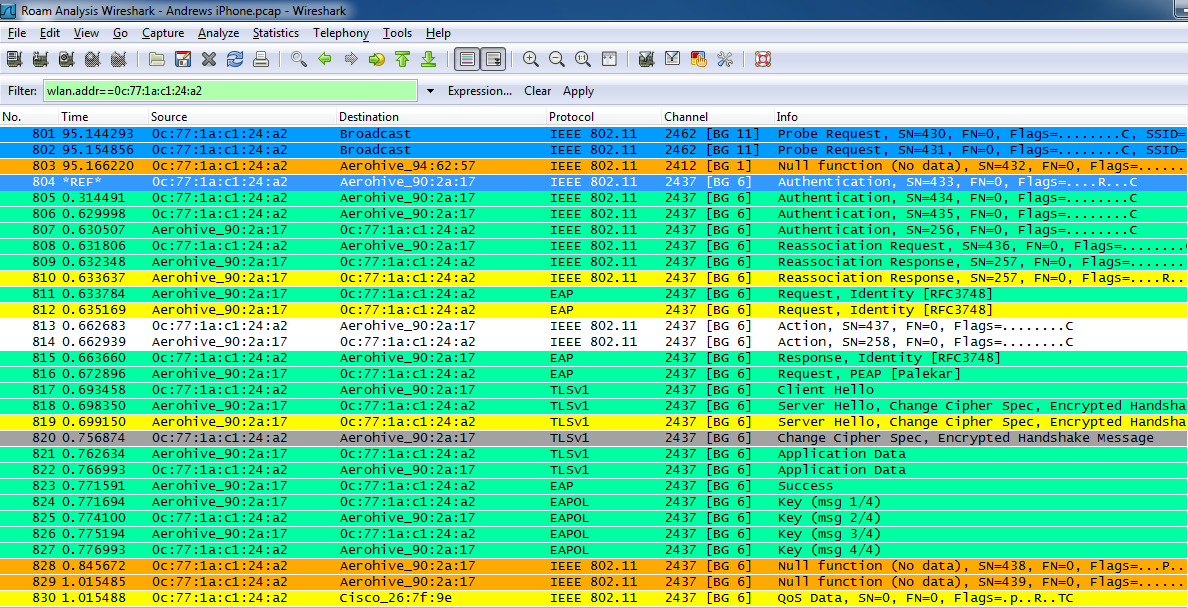
\includegraphics[width=2in]{media/wireshark.png}\;
    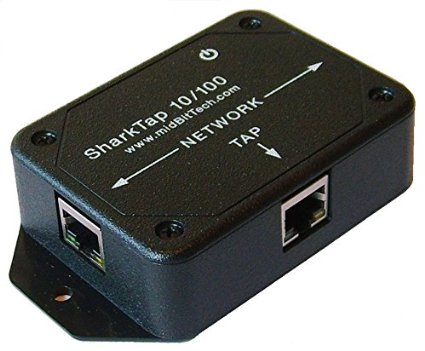
\includegraphics[width=1.4in]{media/shark-hw.jpg}
    \begin{itemize}
        \item программные
        \item программно-аппаратные
    \end{itemize}
\end{frame}

% Slide #4
\begin{frame}{Способы перехвата}
    \begin{itemize}
        \item Обычным «прослушиванием» сетевого интерфейса;

        \item Ответвлением (программным или аппаратным) трафика и направлением
            его копии на сниффер (Network tap);

        \item Через анализ побочных электромагнитных излучений и восстановление
            таким образом прослушиваемого трафика;

        \item Через атаку на канальном 2-ом (MAC-spoofing) уровне;
            
        \item Через атаку на канальном сетевом 3-м (IP-spoofing) уровне.
    \end{itemize}
\end{frame}

% Slide #5
\begin{frame}{tcpdump}
    tcpdump — утилита UNIX (есть клон для Windows), позволяющая перехватывать и
    анализировать сетевой трафик, проходящий через компьютер, на котором
    запущена данная программа.
\end{frame}

% Slide #6
\begin{frame}[fragile]{Просмотр интерфейсов}
    \begin{Verbatim}[fontsize=\scriptsize]
$ sudo tcpdump -D
1.wlan0 [Up, Running]
2.docker0 [Up, Running]
3.vboxnet0 [Up, Running]
4.vboxnet1 [Up, Running]
5.veth283f985 [Up, Running]
6.any (Pseudo-device that captures on all interfaces) [Up, Running]
7.lo [Up, Running, Loopback]
8.eth0 [Up]
9.bluetooth-monitor (Bluetooth Linux Monitor)
10.nflog (Linux netfilter log (NFLOG) interface)
11.nfqueue (Linux netfilter queue (NFQUEUE) interface)
12.usbmon1 (USB bus number 1)
13.usbmon2 (USB bus number 2)
    \end{Verbatim}
\end{frame}

% Slide #7
\begin{frame}[fragile]{Все запросы с интерфейса}
    \begin{Verbatim}[fontsize=\scriptsize]
$ sudo tcpdump -i wlan0
tcpdump: verbose output suppressed, use -v or -vv for full protocol decode
listening on wlan0, link-type EN10MB (Ethernet), capture size 262144 bytes
19:04:24.115872 STP 802.1d, Config, Flags [none], bridge-id 8000.bc:ae:c5:88:91:28.8001, length 35
19:04:24.219665 IP Arkasha-PC.local.bootpc > 255.255.255.255.bootps: BOOTP/DHCP, Request from 00:1b:fc:6c:c2:42 (oui Unknown), length 300
19:04:25.118303 IP x220t.local.32371 > google-public-dns-a.google.com.domain: 29524+ PTR? 255.255.255.255.in-addr.arpa. (46)
19:04:25.186526 IP google-public-dns-a.google.com.domain > x220t.local.32371: 29524 NXDomain 0/1/0 (114)
19:04:25.287550 IP6 fe80::120b:a9ff:fe0c:f638.mdns > ff02::fb.mdns: 0 PTR (QM)? 255.255.255.255.in-addr.arpa. (46)
^C19:04:25.287614 IP x220t.local.mdns > 224.0.0.251.mdns: 0 PTR (QM)? 255.255.255.255.in-addr.arpa. (46)

6 packets captured
50 packets received by filter
0 packets dropped by kernel
    \end{Verbatim}
\end{frame}

% Slide #8
\begin{frame}[fragile]{Фильтр по хосту}
    \begin{Verbatim}[fontsize=\scriptsize]
$ sudo tcpdump host readthedocs.org
tcpdump: verbose output suppressed, use -v or -vv for full protocol decode
listening on wlan0, link-type EN10MB (Ethernet), capture size 262144 bytes
19:08:24.734572 IP x220t.local.44169 > readthedocs.org.http: Flags [S], seq 1630487586, win 14600, options [mss 1460,sackOK,TS val 281681188 ecr 0,nop,wscale 7], length 0
19:08:24.900671 IP readthedocs.org.http > x220t.local.44169: Flags [S.], seq 2780774205, ack 1630487587, win 14480, options [mss 1460,sackOK,TS val 1880995361 ecr 281681188,nop,wscale 9], length 0
19:08:24.900718 IP x220t.local.44169 > readthedocs.org.http: Flags [.], ack 1, win 115, options [nop,nop,TS val 281681229 ecr 1880995361], length 0
19:08:24.900812 IP x220t.local.44169 > readthedocs.org.http: Flags [P.], seq 1:733, ack 1, win 115, options [nop,nop,TS val 281681229 ecr 1880995361], length 732
...
  19:08:28.524595 IP readthedocs.org.https > x220t.local.37282: Flags [.], ack 2254, win 40, options [nop,nop,TS val 1880996266 ecr 281682094], length 0
19:08:28.605826 IP x220t.local.37282 > readthedocs.org.https: Flags [.], ack 9767, win 296, options [nop,nop,TS val 281682155 ecr 1880996287], length 0
^C
83 packets captured
89 packets received by filter
0 packets dropped by kernel
    \end{Verbatim}
\end{frame}

% Slide #9
\begin{frame}[fragile]{Ещё фильтры}
    По протоколу:
    \begin{Verbatim}[fontsize=\scriptsize]
$ sudo tcpdump -n tcp
    \end{Verbatim}
    По назначению:
    \begin{Verbatim}[fontsize=\scriptsize]
$ sudo tcpdump -n 'src 192.168.1.101'
    \end{Verbatim}
    Только DNS пакеты:
    \begin{Verbatim}[fontsize=\scriptsize]
$ sudo tcpdump -n 'udp and dst port 53'
tcpdump: verbose output suppressed, use -v or -vv for full protocol decode
listening on wlan0, link-type EN10MB (Ethernet), capture size 262144 bytes
19:22:52.089174 IP 192.168.1.101.17166 > 8.8.8.8.53: 44241+ A? www.google.ru. (31)
19:22:52.149972 IP 192.168.1.101.61715 > 8.8.8.8.53: 63972+ A? www.google.ru. (31)
19:22:52.157017 IP 192.168.1.101.12023 > 8.8.8.8.53: 17412+ AAAA? www.google.ru. (31)
19:22:54.062859 IP 192.168.1.101.30447 > 8.8.8.8.53: 54230+ AAAA? www.google.ru. (31)
    \end{Verbatim}
\end{frame}

% Slide #10
\begin{frame}[fragile]{Поиск хостов}
    NetBIOS:
    \begin{Verbatim}[fontsize=\scriptsize]
$ nbtscan 192.168.1.0/24
Doing NBT name scan for addresses from 192.168.1.0/24

IP address       NetBIOS Name     Server    User             MAC address
------------------------------------------------------------------------------
192.168.1.0     Sendto failed: Permission denied
192.168.1.101    X220T            <server>  X220T            00:00:00:00:00:00
192.168.1.23                      <server>                   00:00:00:00:00:00
192.168.1.22     ARKASHA-PC       <server>  <unknown>        00:1b:fc:6c:c2:12
192.168.1.255   Sendto failed: Permission denied
    \end{Verbatim}
    Nmap:
    \begin{Verbatim}[fontsize=\scriptsize]
$ nmap -sP 192.168.1.*

Starting Nmap 6.46 ( http://nmap.org ) at 2015-02-02 20:56 YEKT
Nmap scan report for 192.168.1.1
Host is up (0.0068s latency).
Nmap scan report for 192.168.1.20
Host is up (0.018s latency).
Nmap scan report for 192.168.1.21
Host is up (0.016s latency).
    \end{Verbatim}
\end{frame}

% Slide #11
\begin{frame}[fragile]{Трафик между двух узлов сети}
    Только ICMP пакеты (ping)
    \begin{Verbatim}[fontsize=\scriptsize]
$ sudo tcpdump 'src 192.168.1.101 and dst 192.168.1.23 and icmp'
tcpdump: verbose output suppressed, use -v or -vv for full protocol decode
listening on wlan0, link-type EN10MB (Ethernet), capture size 262144 bytes
19:36:45.340321 IP x220t.local > 192.168.1.23: ICMP echo request, id 10305, seq 1, length 64
19:36:46.341472 IP x220t.local > 192.168.1.23: ICMP echo request, id 10305, seq 2, length 64
19:36:47.342180 IP x220t.local > 192.168.1.23: ICMP echo request, id 10305, seq 3, length 64
19:36:48.343557 IP x220t.local > 192.168.1.23: ICMP echo request, id 10305, seq 4, length 64
^C
4 packets captured
4 packets received by filter
0 packets dropped by kernel
    \end{Verbatim}
\end{frame}

% Slide #12
\begin{frame}[fragile]{Поиск в трафике}
    HTTP ответы со статусом 200
    \begin{Verbatim}[fontsize=\scriptsize]
$ sudo tcpdump -n -A | grep -e '200 OK'
tcpdump: verbose output suppressed, use -v or -vv for full protocol decode
listening on wlan0, link-type EN10MB (Ethernet), capture size 262144 bytes
A).)...sHTTP/1.1 200 OK
A).9...vHTTP/1.1 200 OK
    \end{Verbatim}
\end{frame}

% Slide #13
\begin{frame}[fragile]{Поиск логинов и паролей}
    \begin{Verbatim}[fontsize=\scriptsize]
$ sudo tcpdump -l -A -i lo | egrep -i 'pass=|pwd=|log=|login=|user=
    |username=|pw=|passw=|passwd=|password=|pass:|user:|username:
    |password:|login:|pass |user ' --color=auto --line-buffered -B20
tcpdump: verbose output suppressed, use -v or -vv for full protocol decode
listening on lo, link-type EN10MB (Ethernet), capture size 262144 bytes
Host: localhost:6543
User-Agent: Mozilla/5.0 (X11; Ubuntu; Linux x86_64; rv:35.0) Gecko/20100101 Firefox/35.0
Accept: text/html,application/xhtml+xml,application/xml;q=0.9,*/*;q=0.8
Accept-Language: en-US,en;q=0.5
Accept-Encoding: gzip, deflate
Referer: http://localhost:6543/login/
Cookie: csrftoken=pVVycxJs2YaTCS5vpKTob0TINGsKjAM4; _LOCALE_=ru; _ga=GA1.1.1951453052.1420403120; connect.sid=s%3AnGU-04XqEDWudttY3CHI3LdUmEr__MYG.GF2fEjoSwB0bC99vfK%2FibenygTjwjRPLto948y7FSwU; beaker.session.id=27aa2050fff646b5bfe5cce56dae1472
Connection: keep-alive
Content-Type: application/x-www-form-urlencoded
Content-Length: 53

came_from=%2F&login=admin&password=123&submit=Sign+In
    \end{Verbatim}
\end{frame}

% Slide #14
\begin{frame}{Wireshark}
    \begin{center}
        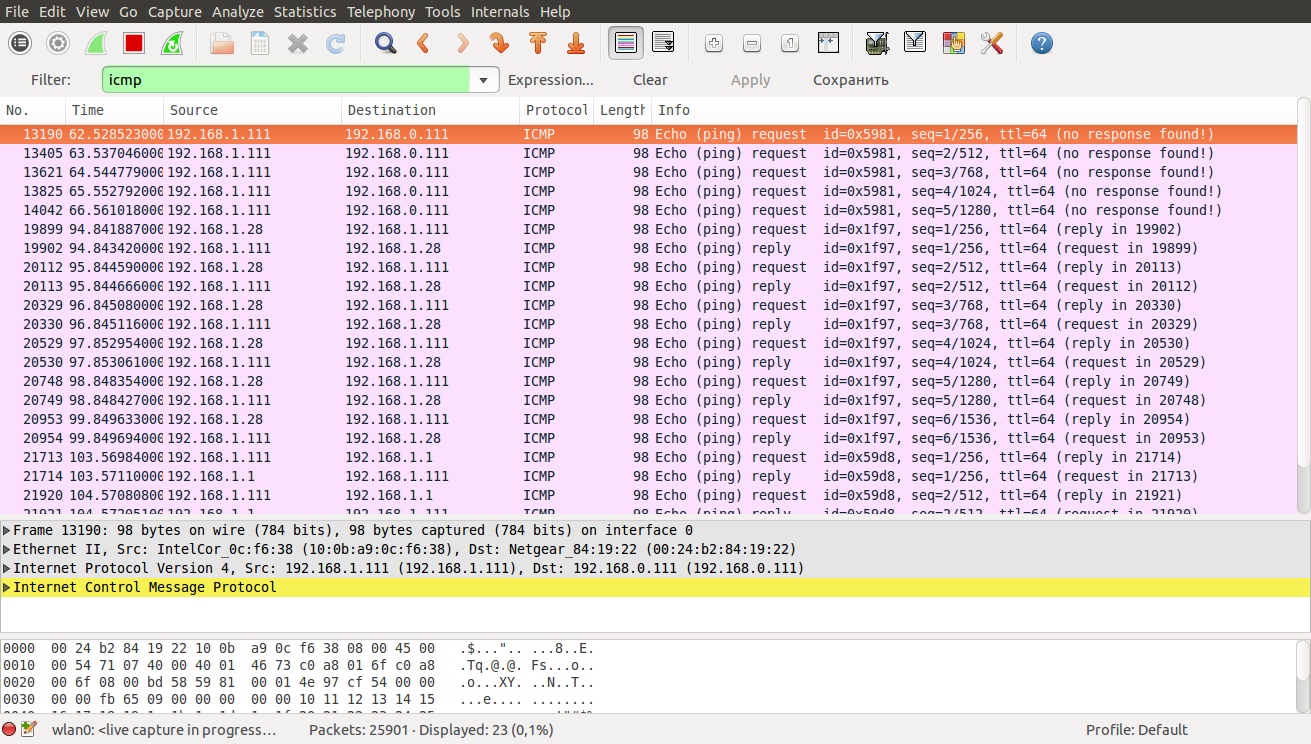
\includegraphics[width=4.2in]{media/wireshark-2.png}
    \end{center}
\end{frame}

\end{document}
